\section{Markov Chains}
\subsection{Markov Processes or Markov Chains}
A Markov chain is simply a Markov Decision Process without decision. It is one the 
most simplest stocastic process, and has no ``memory'' of the past. So, just the 
present stat determines its future dynamics. In this context, we will be considering
Discrete Time Markov Chains (DTMCs).

DTMC involves two concepts:
\begin{itemize}
    \item Discrete Time Stochastic Process (DTSP)
    \item Row Stochastic Matrix.
\end{itemize}

The two are defined as follows:

\begin{definition}[Discrete Time Stochastic Process (DTSP)]
    A DTSP is a sequence \({(X_n)}_{n \geq 0}\) of random variables defined on the same proboability space
    \((\Omega, \mathcal{F} , \mathbb{P} )\), taking values in the same 
    set \(\mathcal{S} \), i.e.
    \[
        X_n : \Omega \rightarrow \mathcal{S} \quad \forall n \geq 0
    \]
\end{definition}
where \(\mathcal{S} \) is called a state space, and in finite or countably infinite.
We call the a variable as a ``state'' when the state is an element of the state space \(\mathcal{S} \).
The cardinality of the state space is denoted by \(|\mathcal{S} |\).

\begin{definition}[Row Stochastic Matrix]
    A matrix \(\mathcal{P} \in \mathbb{R}^{|S| \times |S|}\) is called a row stochastic matrix if
    it satisfies the following conditions:
    \[
        \mathcal{P} _{ij} \in [0, 1] \quad \forall i, j \in \mathcal{S}  
    \]
    \[
        \sum\limits_{j = 1 }^{ |\mathcal{S}|} \mathcal{P} _{ij} = 1 \quad \forall i \in \mathcal{S}  
    \]
\end{definition}
Thus, with these two definitions we can define a Markov Chain (or DTMC) as follows:
\begin{definition}[Markov Chain]
    Let \(\mathcal{S} \) be a finite state space, and \(\nu\) be a distribution over \(\mathcal{S} \).
    \[
        \nu = (\nu _{1}, \nu _{2}, \dots, \nu _{|\mathcal{S}|}) \quad
        \text{s.t} \quad \nu _{i} \in [0, 1] \; \forall i \in \mathcal{S},
        \quad \sum\limits_{i \in \mathcal{S} } \nu _{i} = 1
    \]  
    Further, let \(\mathcal{P} \) be a row stocastic matrix over \(\mathcal{S} \).
    
    Then a DTSP \({(X_n)}_{n \geq 0}\) is called a Markov Chain with initial distribution \(\nu \)
    and transition matrix \(\mathcal{P} \) if it satisfies the following conditions:
    \begin{itemize}
        \item Initial state is distributed according to \(\nu \), i.e.
        \[
            \mathbb{P}(X_0 = i) = \nu _{i} \quad \forall i \in \mathcal{S}    
        \]
        \item Present is independent of the past given the present.
        \[
            \begin{aligned}
                \mathbb{P} \left( 
                    X_{n+1} = i_{n+1} | X_{n} = i_{n}, X_{n-1} = i_{n-1}, \dots, X_{0} = i_{0}
                 \right) &= \mathbb{P} \left( 
                     X_{n+1} = i_{n+1} | X_{n} = i_{n}
                  \right) \\
                    & = \mathcal{P}_{i_{n} i_{n+1}} \quad \forall n \geq 0
            \end{aligned}
        \]
    \end{itemize}
\end{definition}

\begin{example}[Markov Chains]
    Let a Markov chain be defined as follows:
    \[
        \mathcal{S}  = \{1,2\} \quad \nu = (p, 1-p) \quad \mathcal{P}  = \begin{bmatrix}
            1-\alpha  &  \alpha  \\
            \beta  &  1-\beta  \\
        \end{bmatrix}
    \]
    \begin{center}
        \begin{tikzpicture}[->,>=stealth',shorten >=2pt,line width=0.5pt,node distance=2cm]
            \node[circle,draw] (zero) {1};
            \node[circle,draw] (one) [right of=zero] {2};
            \path (zero) edge [loop above] node {\(1-\alpha \)} (zero);
            \path (zero) edge [bend left] node[above] {\(\alpha \)} (one);
            \path (one) edge [loop below] node {\(1-\beta \)} (one);
            \path (one) edge [bend left] node[below] {\(\beta \)} (zero);
        \end{tikzpicture}
    \end{center}
Thus, we can have say:
\[
    \mathbb{P} (X_3 = 1 | X_0 = 1, X_1 = 1 , X_2 - 2) = \beta 
\]

Another example that we can have is:
\[
    \mathcal{S} = \{1,2,3\} \quad \nu = (\nu_{1}, \nu_{2}, \nu_{3}) \quad \mathcal{P} = \begin{bmatrix}
        0 & 1 & 0 \\
        0 & \frac{1}{2} & \frac{1}{2}  \\
        \frac{1}{2} & 0 & \frac{1}{2} \\
    \end{bmatrix}
\]
    \begin{center}
        \begin{tikzpicture}[->,>=stealth',shorten >=2pt,line width=0.5pt,node distance=3cm]
            \node[circle,draw] (one) {1};
            \node[circle,draw] (two) [below right of=zero] {2};
            \node[circle,draw] (three) [below left of=zero] {3};
            \path (one) edge [bend left] node[below left] {\(1 \)} (two);
            \path (two) edge [bend left] node[above] {\(\frac{1}{2} \)} (three);
            \path (three) edge [bend left] node[below right] {\(\frac{1}{2} \)} (one);
        \end{tikzpicture}
    \end{center}
    given, \(\nu = (1,0,0)\), the outcomes of the Markov chain if we sample it are:
    \[
        \begin{aligned}
            X_n &= 1, 2, 3, 3, 1, 2, \dots \\
            &= 1, 2, 3, 1, 2, \dots \\ 
        \end{aligned}
    \] 
\end{example}
\vspace{1em}
Note that, to define the DTMC, we need the initial distribution, but the results wont change on the
choice of the distribution \(\nu\), assuming that the Markov chain is ergodic. Hence, while
defining the markov chain, the initial distribution is not mentioned, and can be assumed
arbitrarily.

\begin{theorem}[Necessary and Sufficient Conditions for DTSP to be Markov Chains]
    A DTSP \({(X_n)}_{n \geq 0}\) on \(\mathcal{S}\)  is a Markov chain \(\langle \mathcal{S} , \mathcal{P} 
    ,\nu \rangle\) if and only if:
    \[
        \mathbb{P} \left( 
            X_{n} = i_{n} , X_{n} = i_{n}, \dots, X_{0} = i_{0}
            \right) = \nu _{i_{0}} \mathcal{P} _{i_{0} i_{1}}
             \mathcal{P} _{i_{1} i_{2}} \dots \mathcal{P} _{i_{n-1} i_{n}} \quad \forall n \geq 0
    \] 
\end{theorem}
\begin{proof}
    To simplify the proof, assume that \(\mathcal{P}_{ij} > 0 \quad \forall i, j \in \mathcal{S} \).
    The theorem remains true in the general case, but requires more book-keeping.

    Suppose, \({(X_n)}_{n \geq 0}\) is a Markov chain \(\langle \mathcal{S} , \mathcal{P}
    , \nu \rangle\). 
    
    Using the fact,
    \[
        \begin{aligned}
            \mathbb{P}(A \cap B) &= \mathbb{P}(A) \mathbb{P}(B | A) \\
            \mathbb{P}(A \cap B \cap C) &= \mathbb{P}(A) \mathbb{P}(B | A) \mathbb{P}(C | A \cap B) \\
        \end{aligned}
    \]
    We get,
    \[
        \begin{aligned}
            \mathbb{P}(X_0 = i_0, \dots , X_n = i_n)  & = \mathbb{P} \left( 
                \{X_0 = i_0\} \cap \{X_1 = i_1\} \cap \dots \cap \{X_n = i_n\}
             \right)\\ 
             & = \mathbb{P}(X_0 = i_0) \mathbb{P}(X_1 = i_1 | X_0 = i_0) \dots \mathbb{P}(X_n = i_n | X_{n-1} = i_{n-1}) \\
             & = \mathbb{P} (X_0 = i_0) \mathbb{P}(X_1 = i_1 | X_0 = i_0) \dots \mathbb{P}(X_n = i_n | X_{n-1} = i_{n-1}) \\
             &\dots  \text{Using the memoeryless property of Markov chains} \\
                & = \nu _{i_0} \mathcal{P} _{i_0 i_1} \dots \mathcal{P} _{i_{n-1} i_n} \\
        \end{aligned}
    \]

    This proves the forward claim. To show the reverse claim:

    Put \(n=0\), in the claim, to trivially get the initial distribution back, showing one part of the definition.
    For the other part:
    \[
    \begin{aligned}    
        \mathbb{P}(X_{n} = i_{n} | X_{n-1} = i_{n-1}, \dots, X_{0} = i_{0}) &=
         \frac{\mathbb{P}(X_{n} = i_{n}, \dots, X_{0} = i_{0})}
         {\mathbb{P}(X_{n-1} = i_{n-1}, \dots, X_{0} = i_{0})} \\
         &= \frac{\nu _{i_0} \mathcal{P} _{i_0 i_1} \dots \mathcal{P} _{i_{n-1} i_n}}
         {\nu _{i_0} \mathcal{P} _{i_0 i_1} \dots \mathcal{P} _{i_{n-1} i_n}} \\
            &= \mathcal{P} _{i_{n-2} i_{n-1} } \\
    \end{aligned}
    \]

    Now we need to show:
    \[
        \mathbb{P}(X_{n} = i_{n} | X_{n-1} = i_{n-1})
    \]
    \[
        \begin{aligned}
            & = \frac{\mathbb{P}(X_{n-1} = i_{n-1}, X_{n} = i_{n})}{\mathbb{P}(X_{n-1} = i_{n-1})} \\
            & = \frac{\sum_{i_0 \in \mathcal{S} } \mathbb{P}(X_0 = i_0 \dots  X_{n-1} = i_{n-1}, X_{n} = i_{n})}
            {\sum_{i_0 \in \mathcal{S} } \mathbb{P}(X_{n-1} = i_{n-1}, X_{0} = i_{0})} \\
            & = \mathcal{P} _{i_{n-1} i_n} \\
        \end{aligned}
    \]
\end{proof}\vspace{1em}
In the above proof we have used the following series of fact:
\[
    \begin{aligned}
        \mathbb{P} (X_2 = j) & = \mathbb{P}(\Omega \cap \{X_2 = j\})\\
        &= \mathbb{P} \left[ 
            \bigcup_{i=1}^{ |S| } \{X_i = i\} \cap \{X_2 = j\}
         \right] \\
    \end{aligned}
\]
Using the fact:
\[
    (A \cup B) \cap C = (A \cap C ) \cup (B \cap C)
\]
we get:
\[
    \begin{aligned}
        \mathbb{P} (X_2 = j) & = \sum\limits_{i = 1}^{ |S| } 
        \mathbb{P} \left(
             X_i = i, X_2 = j
         \right)
    \end{aligned}
\]

\begin{theorem}[Markov Property]
    Let \({(X_n)}_{n \geq  0} \) be the markov chain detnoted by \(\langle \mathcal{S} ,\mathcal{P} ,\mu  \rangle \),
then condintional on \(\{X_m = i\}\), \(\{X_{m+n} \}\) is the markov chain \(\langle \mathcal{S} ,\mathcal{P} , \delta _i \rangle \) 
and is independent of \(X_1, X_2, \dots , X_m\), where \(\delta _i\) is the distribution that is 1 at \(i\)
 and 0 everywhere else, i.e
 \[
        \delta _i (j) \equiv \delta_{ij} =  \begin{cases}
            1 & \text{if } j = i \\
            0 & \text{otherwise} \\
        \end{cases} 
 \]
\end{theorem}
\begin{proof}
    It suffices to show the following, for any \(n \geq 0\) and on an event \(A\), related to \(X_0,\dots , X_m\):
    \[
        \begin{aligned}
            \mathbb{P} \left[ 
                (X_m = i_m, X_{m+1} = i_{m+1}, \dots , X_{m+n} = i_{m+n}) \cap A \mid X_m = i_m 
                \right] \\ 
                = \mathbb{P} ( A \mid X_m=i_m) \delta_{ij} \mathcal{P} _{i_m i_{m+1}} \dots 
                \mathcal{P} _{i_{m+n-1} i_{m+n}} 
            \end{aligned}
    \]
    The above equation is just conditional independence:
    \[
        \mathbb{P} (E_1 \cap  E_2 \mid X_m = i) = \mathbb{P} (E_1 \mid X_m = i) \mathbb{P} (E_2 \mid X_m = i)
    \]
    where \(E_2 = (X_m = i_m, X_{m+1} = i_{m+1}, \dots , X_{m+n} = i_{m+n})\) and \(E_1 = A\). The proof of the above statement goes as follows:

    Let \(A\) be an elementary event, i.e. \(A = \{X_0 = j_0, X_1 = j_1, \dots , X_m = j_m\}\). Consider the LHS of the above equation:
    Then, we have two cases:
    \begin{itemize}
        \item \textbf{Case 1}: \(j_m \neq i_m\). Then, the LHS is trivially 0, since \(A\) and \(E_2\) are disjoint.
        \item \textbf{Case 2}: \(j_m = i_m\). Then, we have further cases. When, \( i \neq i_m = j_m\), then 
        the LHS and RHS are again 0. But when \(i = i_m = j_m\), then the LHS is: 
        \begin{multline*}
        \begin{aligned}
                \mathbb{P} (
                    X_0 = j_0, X_1 = j_1, \dots X_m = j_m = i ,X_m = i_m = i, X_{m+1} = i_{m+1},\\ \dots , X_{m+n} = i_{m+n} \mid X_m = i_m = i 
                    )
                \end{aligned}
            \end{multline*}
            \[
                \begin{aligned}
                    &= \frac{\nu(j_o) \mathcal{P}_{j_0 j_1} \dots \mathcal{P}_{j_{m-1} j_m} 
                    \mathcal{P}_{j_m i_{m+1}} \dots \mathcal{P}_{i_{m+n-1} i_{m+n}}}
                    {\mathbb{P} (X_m = i_m = i)} \\
                    &= \frac{\mathbb{P} (A) \mathcal{P}_{i_m i_{m+1}} \dots \mathcal{P}_{i_{m+n-1} i_{m+n}}}
                    {\mathbb{P} (X_m = i_m = i)} \\
                    &= \mathbb{P} (A \mid X_m = i_m = i) \mathcal{P}_{i_m i_{m+1}} \dots \mathcal{P}_{i_{m+n-1} i_{m+n}} \\
                \end{aligned}
            \]
            \end{itemize}
    Thus, completing the proof. This can be extended to non elementary event \(A\) by using the fact that
    any event \(A\) can be written as a union of elementary events, i.e
    \[
        A = \bigcup_{i=1}^{ |S| } \{X_0 = i_0, X_1 = i_1, \dots , X_m = i_m\}
    \]
\end{proof}

\begin{theorem}[Linear Algebra and Markov Chains]
    Let \({(X_n)}_{n \geq 0}\) be the marrkov chain \(\langle \mathcal{S} , \mathcal{P} , \nu \rangle\).
    Then:
    \begin{enumerate}
        \item \(\mathbb{P} (X_n = j) = {(\nu \mathcal{P} ^{n})}_{j} \)
        \item \(\mathbb{P}_i (X_n = j) = \mathbb{P} \left( X_{m+n} = j \mid X_m = i \right) 
        = \mathcal{P}_{ij}^{(n)}\equiv \text{ij entry of } \mathcal{P} ^{n}\)
    \end{enumerate}
\end{theorem}
\begin{proof}
    The second statement is obivious from the first statement. The proof of the first statement goes as follows:

    \textbf{Proof by induction}: For \(n=0\), we have:
    \[
        \mathbb{P} (X_0 = j) = \nu _j \equiv \nu(j)  
    \]
    Now, assume that the statement is true for \(n\), then we have:
    \[
        \begin{aligned}
            \mathbb{P} (X_{n+1} = j) &= \mathbb{P} \left( 
                \bigcup_{i=1}^{ |S| } \{X_n = i , X_{n+1} = j\}
             \right) \\
                &= \sum_{i=1}^{ |S| } \mathbb{P} (X_n = i, X_{n+1} = j) \\
                &= \sum_{i=1}^{ |S| } \mathbb{P} (X_n = i) \mathbb{P} (X_{n+1} = j \mid X_n = i) \\
                &= \sum_{i=1}^{ |S| } \mathbb{P} (X_n = i) \mathcal{P}_{ij} \\
                &= \sum_{i=1}^{ |S| } {(\nu \mathcal{P}^n)}_j \mathcal{P}_{ij} \\
                &= {(\nu \mathcal{P}^{n+1})}_j \\
        \end{aligned}
    \]
    Thus, the proof is complete.
\end{proof}

\subsection{Communicating Classes}
\begin{definition}
    Let \(\langle \mathcal{S} , \mathcal{P} , \nu \rangle\) be a markov chain. Then, we say \(i\) leads to 
    \(j\) denoted as \(i \to j\) if:
    \[
        \mathbb{P}_i ( X_n = j \text{ for some } n \geq 0) > 0
    \] 
    which is equivalent to:
    \[
        \mathbb{P}( X_{m+n} = j \text{ for some } n \geq 0 \mid X_m = i) > 0
    \]
\end{definition}
\begin{definition}
    Let \(\langle \mathcal{S} , \mathcal{P} , \nu \rangle\) be a markov chain. Then, we say \(i\) and \(j\) communicate
    denoted as \(i \leftrightarrow j\) if:
    \[
        i \to j \text{ and } j \to i
    \]
\end{definition}
\begin{theorem}
    The following statements are equivalent:
    \begin{itemize}
        \item \(i \leftrightarrow j\)
        \item \(\mathcal{P}_{i_0 i_1} \mathcal{P}_{i_1 i_2} \dots \mathcal{P}_{i_{n-1} i_n} > 0 \)
        for some \(n \geq  0\)  and some sequence of states \(i_0, i_1, \dots , i_n\)
         such that \(i_0 = i\) and \(i_n = j\).
         \item \(\mathcal{P}_{ij}^{(n)} > 0 \text{ for some } n \geq 0\)
    \end{itemize}
\end{theorem}
\begin{proof}
    i did not understood this :( Revisit this later.
\end{proof}
\begin{definition}[Communicating Class]
    Each equivalence class of the relation \(\leftrightarrow\) is called a communicating class.

    A communicating class is called closed if \(\forall i \in C, i \to j \implies j \in C\).
\end{definition} 

\begin{example}\label{ex:commclass}
    The properties that hold in this example are:\\
    \begin{center}
        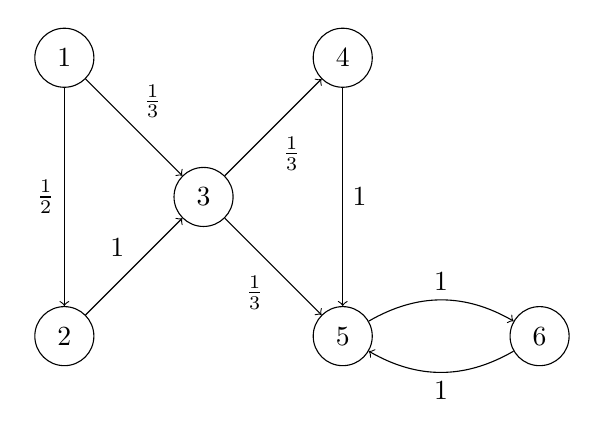
\begin{tikzpicture}[
            node distance=2.5cm,
            state/.style={circle, draw, fill=white, minimum size=0.75cm},
            ]
            \node (S1) [state] {$1$};
            \node (S3) [below right of=S1] [state] {$3$};
            \node (S2) [below left  of=S3] [state] {$2$};
            \node (S4) [above right of=S3] [state] {$4$};
            \node (S5) [below right of=S3] [state] {$5$};
            \node (S6) [right of=S5] [state] {$6$};
            
            \draw[->] (S1) edge node[left] {$\frac{1}{2}$} (S2);
            \draw[->] (S1) edge node[above right] {$\frac{1}{3}$} (S3);
            \draw[->] (S2) edge node[above left] {$1$} (S3);
            \draw[->] (S4) edge node[right] {$1$} (S5);
            \draw[->] (S3) edge node[below right] {$\frac{1}{3}$} (S4);
            \draw[->] (S3) edge node[below left] {$\frac{1}{3}$} (S5);
            \path[->] (S5) edge [bend left] node[above] {\(1\)} (S6);
            \path[->] (S6) edge [bend left] node[below] {\(1\)} (S5);
            % \draw[->, bend angle=45] (S4) edge node[above] {$f$} (S1);
            % \draw[->] (S5) edge node[below] {$g$} (S2);
            % \draw[->] (S5) edge node[right] {$h$} (S6);
            % \draw[->] (S6) edge node[below, sloped] {$i$} (S4);
        \end{tikzpicture}\\
    \end{center}
    \[
        \begin{aligned}
             1 & \leftrightarrow 2 \\
             2 & \leftrightarrow 3 \implies 1 & \leftrightarrow 3 \\
        \end{aligned}
    \]
    We also have the following:
    \[
        \begin{aligned}
            3 & \to  4,5,6 \\
            4 & \to  5,6 \\
            5 & \leftrightarrow 6 \\
        \end{aligned}  
    \]
    Thus, the following can be concluded:
    \[
        \begin{aligned}
        \text{Communicating Classes} &= \{1,2,3\}, \{4\}, \{5,6\}\\
        \text{Closed Groups} &=  \{5,6\}
        \end{aligned}
    \]
\end{example}

\subsection{Strong Markov Property}
\begin{definition}[Stopping Time]
    A random variable \(T : \Omega \rightarrow \{0,1,\dots \} \) is called a stopping time if for any \(n \geq 0\),
    the occurance or non occurance of the event \(\{T = n\}\) can be determined based only on
     the values of \(X_0, X_1, \dots , X_n\).  
\end{definition}
\begin{example} The following are examples of stopping times:
    \item \emph{First passage time}:
    \[
        T_j = \inf \{n \geq 1 : X_n = j\}
    \]
    \item \emph{Last passage time}:
    \[
        T_j = \sup \{n \geq 0 : X_n = j\}
    \]
\end{example}
\begin{definition}[Strong Markov Property]
    Let \((X_n)_{n \geq 0}\) be a markov chain \((\mathcal{S} , \mathcal{P} , \mu )\) and let \(T\), be a stopping
    time. Then, conditional on \(T < \infty \) and \(X_T = i\), the process \((X_{T+n})_{n \geq 0}\) is a markov
    chain with initial distribution \(\delta _i\) and is independent of \(X_0, X_1, \dots , X_T\).
\end{definition}

\subsection{Recurrance and Transience}
Let \((X_n)_{n \geq 0}\) be the markov chain \(\langle \mathcal{S} , \mathcal{P} , \nu \rangle\).
\begin{definition}[Recurrence]
    A state \(i\) is called recurrent if:
    \[
        \mathbb{P}_i (X_i = 1 \text{ for infinitely many } n) = 1
    \] 
\end{definition}
\begin{definition}[Transience]
    A state \(i\) is called transient if:
    \[
        \mathbb{P}_i (X_i = 1 \text{ for infinitely many } n) < 1
    \]
\end{definition}
Loosly, a recurrent state is one that the markov chain keeps visiting, while a transient state is one that
the markov chain never visits from some time on.

\begin{definition}[Passage Time]
    First Passage Time to state \(j\):
    \[
        T_j \coloneqq  \inf \{n \geq 1 : X_n = j\}
    \]
    or,
    \[
        T_j : \Omega \to \{0,1,2,\dots \} \cup \{\infty\}
    \]
    rth passage time to state \(j\): We can define this inductivly as follows:
    \[
        T_j^{(0)} = 0 \implies T_j^{(1)} = T_j
    \]
    \[
        \implies T_j^{(r+1)} = \inf \{n > T_j^{(r)} : X_n = j\}
    \]
    rth excursion or sojorn time:
    \[
        S_j^{(r)} = \begin{dcases}
            T_j^{(r)} - T_j^{(r-1)} & \text{if } T_j^{(r-1)} < \infty \\
            0 & \text{otherwise}
        \end{dcases}
    \]
\end{definition}
\begin{lemma} 
    For \( r = 2,3,\cdots \) condintional on \(T_i^{(r-1)} < \infty \), \(S_i^r\) is independent
    of \(X_m\) for \(0 < m < T_i^{(r-1)}\). Further,
    \[
        \mathbb{P}_i (S_i^r = n \mid T_i^{(r-1)} < \infty) = \mathbb{P}_i(T_i = n)  
    \]
\end{lemma}
\begin{lemmaproof}
    \[
        \{T_i^{(r-1)}\} \subseteq \{X_{T_i^{(r-1)}}\}
    \]
    \[
        \therefore \{T_i^{(r-1)}\} = \{T_i^{(r-1)}\} \cap \{X_{T_i^{(r-1)}} = i\}
    \]
    This implies conditioning on the event \(\{T_i ^{(r-1)} < \infty \} \) is equivalent
    to conditioning on \(\{T_i^{(r-1)}\} < \infty \) and \( \{X_{T_i^{(r-1)}} = i\} \). Further
    \(T_i^{r-1}\) is a stopping time. Thus, conditional on \(\{T_i^{(r-1)} < \infty\} \text{ and } \{
        X_{T_i^{(r-1)} = i}\} \)
    \[
        {\left( 
            X_{T_j^{(r-1)}}
         \right)}_{(n \geq 0)} \text{ is a markov chain } 
    \]
    Now,
    \[
        \mathbb{P} (
            S_i^{(r)} = n \mid T_i^{(r-1)} < \infty
            ) 
    \]
    \[
        \begin{aligned}
                &= \mathbb{P} (S_i^{(r)} = n \mid T_i^{(r-1)} < \infty, X_{T_i^{(r-1)}} = i) \\
                &= \mathbb{P} (
                    X_{T_i^{(r-1)} + 1} \neq i, \dots , X_{T_i^{(r-1)} + n} = i 
                \mid T_i^{(r-1)} < \infty, X_{T_i^{(r-1)}} = i) \\
                &= \mathbb{P} (
                    X_1 \neq i, \dots , X_n = i \mid X_0 = i
                ) \\
                &= \mathbb{P}_i (T_i = n) \\
            \end{aligned}
    \]
    Completing the proof.
\end{lemmaproof}

\begin{definition}[Number of Visits]
    \[
        V_i = \sum_{n=1}^{\infty} \mathbb{I} \{X_n = i\}
    \]
\end{definition}
Thus, we have the following:
\[
    \mathbb{E}_i (V_i) = \mathbb{E}_i \sum_{n=0}^{\infty} \mathbb{I} \{X_n = i\} = 
    \sum_{n=0}^{\infty} \mathbb{P}_i (X_n = i) = \sum _{n=0}^{\infty} \mathcal{P}_{ii}^{(n)}
\]
we can replace the sum with the expectation, using the monotone convergence theorem.
\begin{lemma}
    Let \(f_i \coloneqq \mathbb{P} _i(T_i < \infty )\). Now for \(r = 0,1,\dots \) we have:
    \[
        \mathbb{P} _i (V_i > r) = f_i^r
    \] 
\end{lemma}
\begin{lemmaproof}
    We can prove this using induction.
    
    Base case: \(r = 0\):
    \[
        r = 0 \implies  \mathbb{P} _i (V_i > 0) = 1 \text{ and }  f_i^0 = 1
    \]
    Thus, the base case holds true trivially.

    Suppose, the given claim holds true for some \(r\). Then,
    \[
        \begin{aligned}
            \mathbb{P} _i (V_i > r+1) &= \mathbb{P}_i (T_i^{(r+1)} < \infty ) \\
            &= \mathbb{P}_i (T_i^{(r)} < \infty, S_i^{(r+1)} < \infty) \\
            &= \mathbb{P}_i (T_i^{(r)} < \infty) \mathbb{P}_i (S_i^{(r+1)} < \infty, T_i^{(r)} < \infty) \\
            &= \mathbb{P} _i (V_i > r) \mathbb{P}_i (T_i < \infty) \\
            &= f_i^r f_i  = f_i^{r+1}
        \end{aligned}
    \] 
\end{lemmaproof}
Thus, using the above lemmas we can state the following theorem:
\begin{theorem}
    Let \((X_n)_{n \geq 0}\) be the markov chain \(\langle \mathcal{S} , \mathcal{P} , \nu \rangle\).
    Then,
    \begin{itemize}
        \item for \(i \in \mathcal{S} \), \(\mathbb{P}_i (T_i < \infty)  = 1 \implies i\) is recurrent, and
        \[
            \sum_{n = 0}^{\infty} \mathcal{P}_{ii}^{(n)} = \infty  
        \]
        \item for \(i \in \mathcal{S} \), \(\mathbb{P}_i (T_i < \infty)  < 1 \implies i\) is transient, and
        \[
            \sum_{n = 0}^{\infty} \mathcal{P}_{ii}^{(n)} < \infty
        \]
    \end{itemize}
\end{theorem}
\begin{proof}
    Consider the case of recurrence. We have:
    \[
        \mathbb{P} _i (V_i = \infty ) = \mathbb{P} _i \left( 
            \bigcap_{r=1}^{\infty} \{V_i > r\}
         \right) 
    \]
    Since, \(\{V_i > r\} \supseteq \{V_i > r+1\}\), using the continuity of probability measure, we get:
    \[
        \mathbb{P}_i (V_i = \infty) = \lim_{r \to \infty} \mathbb{P}_i (V_i > r) = \lim_{r \to \infty} f_i^r = 1
    \]
    \[
        \implies \mathbb{E} _i (V_i) = \infty \implies \sum_{n=0}^{\infty} \mathcal{P}_{ii}^{(n)} = \infty
    \]
    Now, consider the case of transience. Suppose, \(f_i = \mathbb{P}_i(T_i < \infty ) < 1\). Then, we have:
    \[
        \sum_{n=0}^{\infty} \mathcal{P}_{ii}^{(n)} = \sum_{n=0}^{\infty}
         \mathbb{P}_i(T_i = n) = \sum_{n=0}^{\infty} f_i^n = \frac{1}{1-f_i} < \infty
    \]
    Hence, \(\mathbb{P}_i (V_i = \infty) = 0\), which implies that \(i\) is transient. 
\end{proof}

\begin{theorem}
    Let \(C\) be a communicating class in a Markov Chain. Then either all states in \(C\)
    are recurrent or all states in \(C\) are transient.
\end{theorem}
\begin{proof}
    Let \(C\) be a communicating class. Suppose \(i \in C\) is transient.
    \[
        \implies \sum_{n=0}^{\infty} \mathcal{P}_{ii}^{(n)} < \infty
    \]
    Let \(j \in C \text{ and }  \exists n,m \geq 0 \) such that \(\mathcal{P}_{ij}^{(n)} > 0\) and \(\mathcal{P}_{ji}^{(m)} > 0\).
    Then, for \(r \geq  0\):
    \[
        \mathcal{P}_{jj}^{(n+m+r)} \geq \mathcal{P}_{ji}^{(m)} \mathcal{P}_{ii}^{(r)} \mathcal{P}_{ij}^{(n)}
    \]
    \[
        \implies \mathcal{P}_{jj}^{(r)} \leq \frac{\mathcal{P}_{ii}^{(n + r + m)}}
        {\mathcal{P}_{ii}^{(n)} \mathcal{P}_{ii}^{(m)}}
    \]
    \[
        \implies \sum\limits_{r=0}^{\infty} \mathcal{P}_{jj}^{(r)} \leq \frac{\sum_{r=0}^{\infty} \mathcal{P}_{ii}^{(n + r + m)}}
        {\mathcal{P}_{ij}^{(n)} \mathcal{P}_{ji}^{(m)}} < \infty
    \]
\end{proof}
Note that recurrence or transience is a class property. And thus the following theorem can be stated:
\begin{theorem}
    Every recuurent class must be closed. And, Every finite closed class is recurrent.
\end{theorem}
Note that, infinite closed classes need not be necessarily recurrent. The classic random walk on a line of
intergers is a classic example.

\subsection{Invariant Distributions}
\begin{definition}[Invariant Distribution]
    A distribution \(\Pi\) on \(\mathcal{S}\) is called invariant for the markov chain \(\langle \mathcal{S} , \mathcal{P} , \nu \rangle\)
    if:
    \[
        \Pi = \Pi \mathcal{P}
    \]
\end{definition}
Thus, a stationery distribution is a left eigenvector of the transition matrix \(\mathcal{P}\) with eigenvalue 1.
Note that in contrast to linear algebra, vectors are represented as row vectors.
\begin{theorem}
    Let \({(X_n)}_{n \geq 0}\) be the markov chain \(\langle \mathcal{S} , \mathcal{P} , \nu \rangle\).
    Then \({X_{m+n} }_{n \geq 0}\) is also a markov chain with the distribution \(\langle \mathcal{S}
     , \mathcal{P} , \Pi \rangle\), where \(\Pi\) is the invariant distribution of \(\mathcal{P}\).
\end{theorem}
\begin{proof}
    We know that,
    \[
        \mathbb{P} (X_n = j) = {(\nu \mathcal{P}^n)}_j
        \implies \mathbb{P} (X_n = j) = {(\Pi \mathcal{P}^n)}_j = \Pi_j
    \]
    Now,
    \[
        \mathbb{P} (X_m = i_0, X_{m+1} = i_1, \dots , X_{m+n} = i_n)  
    \]
    \[
        \begin{aligned}
            & = \mathbb{P} (X_m = i_0) \mathbb{P} (X_{m+1} = i_1 \mid X_m = i_0) 
            \dots \mathbb{P} (X_{m+n} = i_n \mid X_{m+n-1} = i_{n-1}) \\
            & = \Pi_{i_0} \mathcal{P}_{i_0 i_1} \dots \mathcal{P}_{i_{n-1} i_n} \\
        \end{aligned}
    \]
    \(\implies \left( X_{m+n} \right)_{n \geq 0}\) is a markov chain with the distribution \(\Pi \)  
\end{proof}

\begin{theorem}
    Every markov chain on a finite set space has at least one invariant distribution.
\end{theorem}
\begin{proof}
    Since \(\mathcal{P} \) is a row stocastic matrix:
    \[
        \mathcal{P} \mathbf{1} = \mathbf{1}  
    \]
    Since \(\mathcal{P} \) and \(\mathcal{P} ^{\top} \) have the same eigenvalues, we have:
    \[
        \implies \exists \nu  \neq 0 \text{ such that }  \nu \mathcal{P} = \nu
    \]
    Since, \(\mathcal{P}\) is a real valued matrix, taking the complex conjugate of the above equation, we get:
    \[
        \overline{\nu} \mathcal{P} = \overline{\nu}
    \]
    Thus, adding and subtracting the above two equations, we get:
    \[
        \Re (\nu) \mathcal{P} = \Re (\nu) \quad \text{ and } \quad  \Im (\nu) \mathcal{P} = \Im (\nu)
    \]
    Since, \(v \neq  0\), atleast one of \(\Re (\nu) \) or \(\Im (\nu) \) is non zero.
    Thus, if \(\mathcal{P} \) has a complex left eigenvector, then it has a real left eigenvector.

    Now, without loss of generality, let \(u\) be a real valued vector such that:
    \[
        u \mathcal{P} = u
    \]
    Defining,
    \[
        u_+(i) \coloneqq  \max \{u(i), 0\} \quad \text{ and } \quad u_-(i) \coloneqq  \max \{-u(i), 0\}
    \]
    we have:
    \[
        \implies u = u_+ - u_-
    \]
    letting,
    \[
        u_+ \mathcal{P} \eqqcolon u_+ \quad \text{ and } \quad u_- \mathcal{P} \eqqcolon  u_-
    \]
    we get,
    \[
        u \mathcal{P} = u_+ \mathcal{P} - u_- \mathcal{P} = y_+ - y_-  
    \]
    Suppose: \( u_+(i) > 0  \implies  u_-(i) = 0\).
    \[
        \implies y_+(i) - y_-(i) = u_+(i) \implies y_+(i) = u_+(i) \text{ and } y_-(i) = 0 
    \]
    Similiarly
    \[
        u_+(i) = 0 \implies u_-(i) > 0 \implies y_+(i) = 0 \text{ and } y_-(i) = u_-(i)
    \]
    Thus, we can conclude:
    \[
        u_+ \mathcal{P} = u_+ \quad \text{ and } \quad u_- \mathcal{P} = u_-
    \]
    Since \(u \neq  0\), either of \(u_+\) or \(u_-\) is non zero. 
    Thus, we have found a non zero left real valued eigenvector of \(\mathcal{P}\).

    Let \(z\) be the non zero vector among  \(u_+\) or \(u_-\). Then, we have:
    \[
        z \mathcal{P} = z \quad \text{ and } \quad z \neq 0, \; z_i > 0 \implies \sum_{i} z_i > 0 
    \]
    Rescaling the vector we get,
    \[
        \frac{z}{\sum_i z_i} \mathcal{P} = \frac{z}{\sum_i z_i}
    \]
    Defining \(\Pi(i) = \dfrac{z}{\sum_i z_i}\), we get:
    \[
        \Pi \mathcal{P} = \Pi
    \]    
\end{proof}

\begin{definition}
    A markov chain is said tp be irreducible if the whole state space is one communicating class. i.e
    \[
        i \leftrightarrow j \quad \forall\; i,j \in \mathcal{S}
    \]
\end{definition}
\begin{theorem}\label{thm:gamma}
    Let \(\langle \mathcal{S} , \mathcal{P} , \nu \rangle\) be an irreducible
    and recurrent markov chian. Further let 
    \[
        \gamma _i^k = \mathbb{E}_k  \sum_{n=0}^{T_k - 1} \mathbb{I} \{X_n = i\} 
    \]
    and \(\gamma ^k = (\gamma _1^k , \gamma _2^k, \dots , \gamma _{|\mathcal{S}|}^k)\).
    Then, the following holds:
    \begin{enumerate}
        \item \(\gamma ^k_k = 1\)
        \item \(\gamma ^k P = \gamma ^k\)
        \item \(0 < \gamma ^k < \infty\)  
    \end{enumerate}
\end{theorem}
\begin{proof}
    \textbf{(1)}: This is true by the definition of \(\gamma _i^k\).\\
    \textbf{(2)}: We have:
    \[
        \begin{aligned}
            \gamma _j^k &= \mathbb{E}_k  \sum_{n=0}^{T_k - 1} \mathbb{I} \{X_n = j\}\\
            & = \mathbb{E}_k  \sum_{n=1}^{T_k} \mathbb{I} \{X_n = j\} = 
            \mathbb{E}_k  \sum_{n=0}^{\infty } \mathbb{I} \{X_n = j, n \leq T_k\} \\
            & = \sum_{n=1}^{\infty} \mathbb{P}_k (X_n = j, n \leq T_k) \hfill \qquad \text{ //by monotone convergence theorem} \\
            & = \sum_{n=1}^{\infty} \sum_{i \in \mathcal{S}} \mathbb{P}_k (X_n = j, X_{n-1} = i, n \leq T_k) \\
            & = \sum_{n=1}^{\infty} \sum_{i \in \mathcal{S}} \mathbb{P}_k (X_n = j \mid 
            X_{n-1} = i, n \leq T_k) \mathbb{P}_k (X_{n-1} = i, n \leq T_k) \\ 
            & = \sum_{n=1}^{\infty} \sum_{i \in \mathcal{S}} \mathcal{P}_{ij} \mathbb{P}_k (X_{n-1} = i, n \leq T_k) \\
        \end{aligned}
    \]
    Since we are summing over non negative sum, we can interchange the summation. Thus, we get:
    \[
        \begin{aligned}
            \gamma _j^k &= \sum_{i \in \mathcal{S}} \mathcal{P}_{ij} \sum_{n=1}^{\infty} \mathbb{P}_k (X_{n-1} = i, n \leq T_k) \\
            & = \sum_{i \in \mathcal{S}} \mathcal{P}_{ij} 
            \underbrace{\sum_{m=0}^{\infty}\mathbb{P}_k (X_m = i , m \leq T_k - 1)}_
            {\mathbb{E}_k \sum\limits_{m=0}^{T_k - 1} \mathbb{I} \{X_m = i\}} \\
            & = \sum_{i \in \mathcal{S}} \mathcal{P}_{ij} \gamma _i^k
        \end{aligned}
    \]
    \[
        \implies  \gamma ^k \mathcal{P} = \gamma ^k
    \]
    \textbf{(3)}: We will use the fact that the given markov chain is irreducible.
    \[
        \implies \mathcal{P}_{ij}^{(n)} > 0 \quad \forall \; i,j \in \mathcal{S}  
    \]
    Since we know that \(\gamma ^k\) is invariant \(\implies \gamma ^k = \gamma ^k \mathcal{P} = \gamma ^k \mathcal{P}^n\).
    Thus, we have:
    \[
        \gamma ^k_k = \sum_j \gamma _j^{k}\mathcal{P}_{jk}^{(n)} \geq \gamma _i^k \mathcal{P}_{ik}^{(n)}
    \]
    The above statement holds, since sum of non negative quantities is greater than or equal to any of the 
    individual quantities.
    Now,
    \[
        \gamma _k^k = 1 \quad \because \mathcal{P}_{ik}^{(n)} > 0 \implies \gamma _i^k < \infty  
    \]
    Now, to show \(\gamma _i^k > 0\). Let \(\mathcal{P}_{ki}^{(m)} > 0 \)
    \[
        \implies  \gamma _i^k = \sum_j \gamma _j^k \mathcal{P}_{ji}^{(m)} \geq \gamma _k^k \mathcal{P}_{ki}^{(m)}
        = \mathcal{P}_{ki}^{(m)} > 0
    \]
    \[
        \implies 0 < \gamma _i^k < \infty  
    \]
    Completing the proof.
\end{proof}
\begin{theorem}
    Let \(\langle \mathcal{S} , \mathcal{P} , \nu \rangle\) be an irreducible markov chain. Further, let 
    \(\lambda\) be an invariant measure such that \(\lambda _k = 1\), then \(\lambda \geq  \gamma ^k\). If 
    \(\langle \mathcal{S} ,\mathcal{P} ,\nu \rangle \) is additionally recurrent, then \( \gamma^k = \lambda\).
\end{theorem}
\begin{proof}
    NOTE: This theorem also applies with inifinte markov chain.\\
    Since \(\lambda\), is a measure, thus, \(\lambda(i)\) is non negtive. Now, since \(\lambda\) is invariant, we have:
    \[
        \lambda = \lambda \mathcal{P} \implies \lambda(j) = \sum_{i \in \mathcal{S}} \lambda(i) \mathcal{P}_{ij}
        = \sum_{i_1 \neq k} \lambda(i) \mathcal{P}_{ij} + \mathcal{P}_{kj}
    \]
    Massaging \(\mathcal{P}_{kj} \), we get:
    \[
        \mathcal{P}_{kj} = \mathbb{P} (X_1 = j \mid X_0 = k) = \mathbb{P}_k (X_1 = j) = \mathbb{P}_k (X_1 = j, T_k > 1)
    \]
    Thus,
    \[
        \begin{aligned}
            \lambda _j &= \sum_{i_1 \neq k} \sum_{i_2 \in \mathcal{S} } 
            \lambda_{i_2} \mathcal{P}_{i_2 i_1} \mathcal{P}_{i_1 j} + \mathbb{P}_k (X_1 = j, T_k > 1) \\
            & = \sum_{i_1 \neq k} \sum_{i_2 \neq k} \lambda_{i_2} \mathcal{P}_{i_2 i_1}
             \mathcal{P}_{i_1 j} + \mathbb{P}_k (X_1 = j, T_k > 1) + \mathbb{P}_k (X_2 = j, T_k > 2) \\
        \end{aligned}
    \]
    From induction, we get:
    \[
        \begin{aligned}
            \lambda _j &= \underbrace{\text{ some expression }}_{\text{non negative}} +
            \sum_{n=1}^{m} \mathbb{P}_k (X_n = j, T_k > n)\\
            \implies  \lambda _j &\geq \sum_{n=1}^{\infty} \mathbb{P}_k (X_n = j, T_k > n) = \gamma _j^k \hfill 
            \qquad \text{ //by \autoref{thm:gamma}}\\
        \end{aligned}
    \]
    Thus, we have:
    \[
        \lambda \geq \gamma ^k
    \]
    Now, if the markov chain is recurrent, then we have to show that \(\lambda = \gamma ^k\).
    Let \(\mu = \lambda -\gamma ^k\). Thus, \(\mu \mathcal{P} = (\lambda - \gamma ^k) \mathcal{P} = \lambda - \gamma ^k = \mu\).
    Now,
    \[
        \mu _k = \lambda _k - \gamma _k^k = 1 - 1 = 0 \quad \mu = \mu \mathcal{P}
    \]
    Choose \(i,k \in \mathcal{S}\) such that \(\mathcal{P}_{ik}^{(n)} > 0\). Then,
    \[
        \begin{aligned}
            0 = \mu _k &= \sum_{j \in \mathcal{S}} \mu _j \mathcal{P}_{jk}^{(n)} \\
            & \geq \mu _i \mathcal{P}_{ik}^{(n)} \implies \mu _i = 0 \forall \; i \in \mathcal{S}
        \end{aligned}
    \]
    \[
        \implies \mu = 0 \implies \lambda = \gamma ^k
    \]
    Completing the proof.
\end{proof}
\begin{theorem}
    Let \(\langle \mathcal{S} , \mathcal{P} , \nu \rangle\) be a finite irreducible markov chain. Then, \(\Pi\) is 
    unique and \(\Pi _i = \frac{1}{m_i}\), where \(m_i = \mathbb{E}_i (T_i)\).  
\end{theorem}
\begin{proof}
    The intuitive meaning of \(m_i\) is the expected time to return to state \(i\), starting from state \(i\).\\
    Since the markov chain is finite, there exits a invariant distribution \(\Pi\) such that \(\Pi = \Pi \mathcal{P} \).\\
    Now,
    \[
        \pi _k = \sum_{j \in \mathcal{S}} \pi _j \mathcal{P}_{jk}^{(n)} \geq \pi _i \mathcal{P}_{ik}^{(n)} > 0
    \]
    Thus, \(\pi _i > 0\). Now, let \(\lambda \coloneqq \frac{\Pi}{\pi _k}\) Thus, \(\lambda _k = 1\)
    \[
        \implies  \lambda \mathcal{P}  = \frac{1}{\pi _k} \Pi \mathcal{P} = \frac{1}{\pi _k} \Pi = \lambda
    \]
    \[
        \implies \lambda \text{ is an invariant measure } 
    \]
    \(\because\) chain is irreducible and from \autoref{thm:gamma}, \(\lambda = \gamma ^k\)
    \[
        \implies \frac{\Pi}{\pi_k} = \gamma ^k \implies \sum_i \frac{\Pi _i}{\pi _k} = \sum_i \gamma _i^k 
        \implies \frac{1}{\pi_k} = \sum_i \gamma ^k
    \]
    \[
        \because \gamma^k > 0 \implies \pi _k = \frac{1}{\sum\limits_i \gamma ^k}
    \]
    Now,
    \[
        \implies \sum_{i} \gamma _i^k = \sum_{i \in \mathcal{S}}\sum_{n = 1}^{\infty} \mathbb{P}_k (X_n = i, n \leq T_k)
    \]
    Now, sum is over all positive quantities, summation can be interchanged. Thus, we get:
    \[
        \begin{aligned}
            \sum_i \gamma _i^k &= \sum_{n=1}^{\infty}\sum_{i \in \mathcal{S}} \mathbb{P}_k (X_n = i, n \leq T_k)\\
            &= \sum_{n=1}^{\infty} \mathbb{P}_k (T_k \geq n) = \mathbb{E}_k (T_k) = m_k
            \implies \pi _k &= \frac{1}{\mathbb{E}_k (T_k)}
        \end{aligned}
    \]
    Thus, completing the proof.
\end{proof}
\begin{definition}
    A state \(i\), is sais to be a aperiodic if \(\mathcal{P}_{ii} > 0\) for sufficient large \(n\).  
\end{definition}
\begin{lemma}
    \(\langle \mathcal{S} , \mathcal{P} , \sigma  \rangle\) is an irreducible markov chain further, suppose 
    \(k \in \mathcal{S} \) is aperiodic. Thus, every \( i \in \mathcal{S}\), is aperiodic. Infact, 
    \(\mathcal{P}_{ii}^{(n)} > 0, \; \forall i,j \in \mathcal{S}\) for sufficient large \(n\).
\end{lemma}
\begin{theorem}
    Let \(\langle \mathcal{S} , \mathcal{P} , \nu \rangle\) be a finite irreducible and aperiodic markov chain. Then,
    irrespective of the initial distribution, the markov chain converges to the unique invariant distribution \(\Pi\). i.e.
    \[
        \lim_{n \to \infty} \mathbb{P} (X_n = i) = \Pi _i \quad \forall \; i \in \mathcal{S}  
    \]
    Further,
    \[
        \lim_{n \to \infty} \mathcal{P}_{ij}^{(n)} = \Pi _j
    \] 
\end{theorem}